\begin{frame}[fragile]{Concepto del perfilador}

    \begin{columns}
        \begin{column}{0.5\textwidth}
        
            \begin{itemize}
                \item Perfiladores con cámaras CCD. Sensores muy caros
                \item Perfiladores integradores. Complejidad mecánica
            \end{itemize}
        \end{column}
        
        \begin{column}{0.5\textwidth}
            \begin{figure}[H]
            \centering
            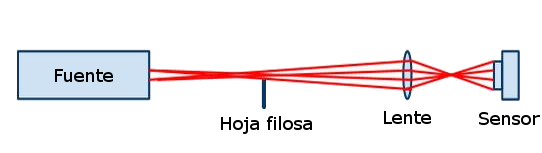
\includegraphics[width=\textwidth]{fig/perfilador/esquema_basico}
            \label{fig:perfilador/esquema_basico}
            \end{figure}
            \begin{figure}
                \centering
                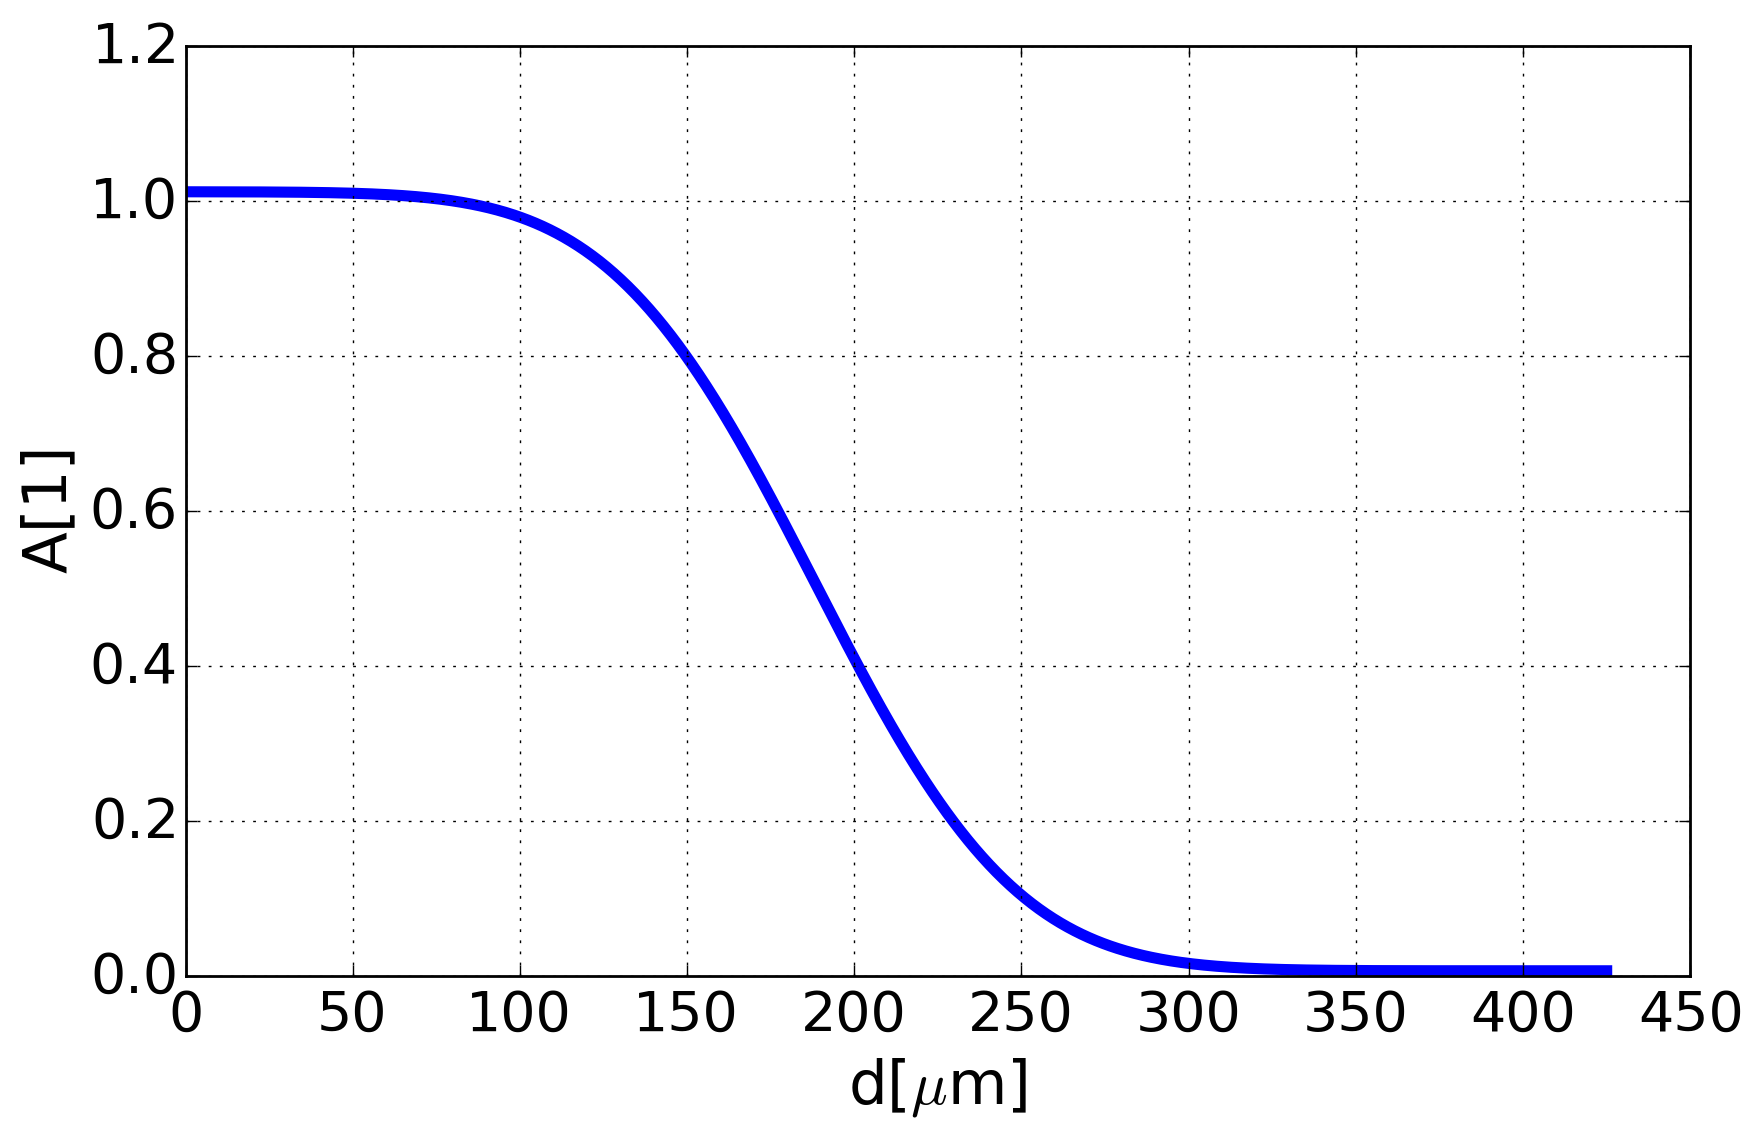
\includegraphics[width=0.8\textwidth]{fig/perfilador/err_function.png}
                \label{fig:perfilador/err_function}
            \end{figure}
        \end{column}
    \end{columns}



\end{frame}

\begin{frame}[fragile]{Concepto del polarizador}
        \begin{figure}[H]
                    \centering
                    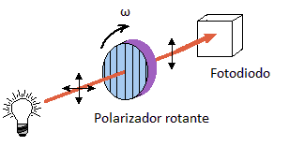
\includegraphics[width=0.5\textwidth]{fig/polarimetro/esquema}
                    %\caption{}
                    \label{fig:polarimetro}
            \end{figure}
        \begin{columns}
            \begin{column}{0.5\textwidth}
                
                \begin{figure}[H]
                    \centering
                    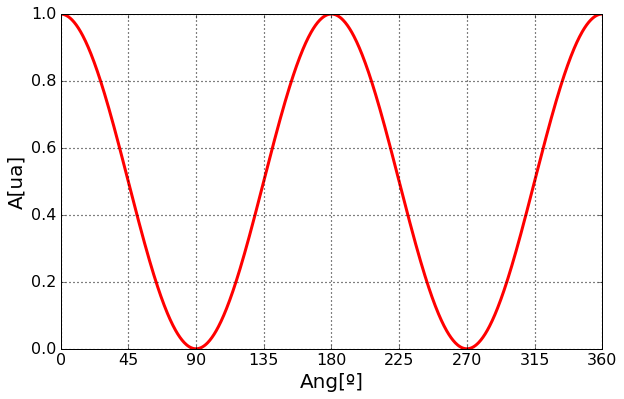
\includegraphics[width=0.7\textwidth]{fig/polarimetro/malus}
                    %\caption{}
                    \label{fig:polarimetro}
                \end{figure}
            \end{column}
            \begin{column}{0.5\textwidth}
                
                \[ \alpha = \frac{\max - \min}{\max + \min} = \begin{cases} 1 & \text{lineal} \\ 0 & \text{circular} \end{cases}\]
            \end{column}
        \end{columns}
   
\end{frame}
